%% You have a maximum of 350, which includes your title, name, etc.
\begin{abstract}
  Atmospheric aerosols play an important role in earth climate change by
scattering and absorbing solar and terrestrial radiation, and indirectly
through altering the cloud formation, lifetime, and radiative
properties. However, accurate quantification of these effects is in no
small part hindered by our limited knowledge about the particle size
distribution and refractive index, the aerosol microphysical properties
essentially pertain to aerosol optical and cloud-forming properties. The
focus of this thesis is the  characterization of aerosol microphysical
properties from ground-based polarimetric remote sensing. 

The central research goal is to obtain accurate aerosol PSD and
refractive index of both fine and coarse modes from the multi-spectral
and multi-agular direct and diffuse solar radiation measured by the
SunPhotometer of Aerosol Robertic Network (AERONET). We do so by (1)
developing an inversion algorithm for the retrieval of aerosol
refractive indices and particle size distribution from a combined use of
direct and diffuse solar radiation measurements from AERONET, (2)
conducting a sensitivity study and error budgeting exercise to examine
the potential of adding polarization to the radiance-only inversion, and
(3) performing ground-based retrievals using available AERONET
polarimetric measurements. 

The results from theoretical information and error analysis show a
remarkable increase in information by adding additional polarization
and/or radiances into the inversion: an overall increase of 2–-5 of DFS
comparing with radiance-only measurements. Correspondingly, smallest
retrieval errors are found in the added-polarization scenario: 2.3\%
(2.9\%) for the fine-mode (coarse-mode) aerosol volume concentration,
1.3\% (3.5\%) for the effective radius, 7.2\% (12\%) for the effective
variance, 0.005 (0.035) for the real part refractive index, and 0.019
(0.068) for the single scattering albedo. These errors represent a
reduction from their counterparts in the radiance-only scenario of 79\%
(57\%), 76\% (49\%), 69\% (52\%), 66\% (46\%), and 49\% (20\%), respectively.
 In real cases, we found that our retrievals are overall consistent with
AERONET operational inversions, but can offer mode-resolved refractive
index and SSA with acceptable accuracy for the aerosol composed by
spherical particles. Along with the retrieval using both radiance and
polarization, we also performed radiance-only retrieval to demonstrate
the improvements by adding polarization in the inversion. Contrast
analysis indicates that with polarization, retrieval error can be
reduced by over 50\% in PSD parameters, 10--30\% in the refractive index,
and 10--40\% in SSA.
\end{abstract}

%% Optional opyrightpage
%\begin{copyrightpage}
%This file may be distributed and/or modified under the conditions of
%the \LaTeX{} Project Public License, either version 1.3c of this license
%or (at your option) any later version.  The latest version of this
%license is in:
%\begin{center}
%   \url{http://www.latex-project.org/lppl.txt}
%\end{center}
%and version 1.3c or later is part of all distributions of \LaTeX version
%2006/05/20 or later.
%\end{copyrightpage}

%% Optional
\begin{dedication}
\begin{center}
  \vskip.6in
  To the memory of my grandfather \\
  \vskip0.2in
\begin{figure}[h]
  \centering
  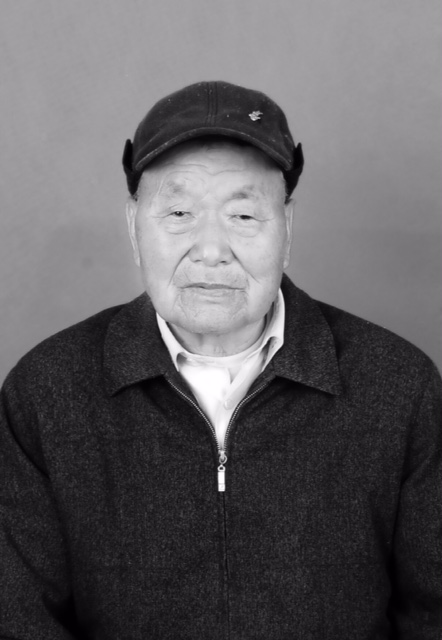
\includegraphics[width={0.35\textwidth}]{figures/grandpapa.jpg}
  \caption*{\textbf{Zhaoxiang Xu} \\
(1933 -- 2014)}
\end{figure}

\end{center}
\end{dedication}

%% Optional
\begin{acknowledgments}
  Acknowledgment to be filled \ldots
\end{acknowledgments}

%% Optional
\begin{grantinfo}
  The NASA Earth and Space Science Fellowship funded this project from September
  2012 to August 2015. I am also grateful to the support
  from NASA's New Investigator Program and Radiation Science Program
  (to Dr. Jun Wang).
\end{grantinfo}
